% !TEX encoding = UTF-8 Unicode
%!TEX root = ../Main/thesis.tex
% !TEX spellcheck = en-US
%%=========================================
\documentclass[../Main/thesis.tex]{subfiles}
\begin{document}
\chapter{Development}\label{ch:development}
In this chapter we will be taking a look at the development in this thesis. The
first section will be focused on learning what the current rebuilder setup is
doing, establish the base requirements of the rewrite of the visualizer with the
goal of improving the design.

After the first iteration is done we will be implementing the Merkle tree
storage for the rebuild submissions which consists of a in-toto link metadata
file, and a BUILDINFO file. Then we will be focusing on implementing the needed
signing of the Merkle tree roots to help verify that the given tree roots
actually comes from the given rebuilder. The final iteration will be the
implementation of the transparency log overlay, which will be the front end for
the APT client to fetch rebuild submission and check if they have been revoked
or not.

The last section deals with the integration between the existing APT transport
and the new visualizer API. We will be removing the support for the old API and
connect it with the new rewritten API with support for transparency logs. We
will then make sure the test suite for the transport completes and everything
works.

\section{Rebuilder}\label{sec:development_rebuilders}
The purpose of the rebuilder is to watch for new packages, queue them, build the
package in a clean environment to reproduce the package, and then publish this
result so we can query these later when installing packages.

To achieve this we need to fulfill a few requirements:

\begin{enumerate}
    \item \label{itm:published} We need to know when a package is published.
    \item \label{itm:scheduler} Something needs to schedule the new packages.
    \item \label{itm:builder} We need to build the package in a clean environment.
    \item \label{itm:publish} We need to publish results of the built package.
    \item \label{itm:transport} We need to check the results when installing packages.
\end{enumerate}

It is important to remember that this system is only targeted at Debian as
supporting it universally would require a lot of engineering effort and handling
of special cases.

\begin{figure}[H]
  \centering
  \begin{sequencediagram}
    \newthread{buildinfo}{buildinfo server}{}
    \newthread{scheduler}{scheduler}{}
    \newthread{redis}{redis}{}
    \newthread{builder}{builder}{}
    \newthread{visualizer}{visualizer}{}
    \begin{call}{scheduler}{NewBuildinfo()}{buildinfo}{}\end{call}

    \begin{call}{scheduler}{rpush}{redis}{}
        \postlevel
    \end{call}

    \prelevel\prelevel
    \setthreadbias{east}

    \begin{call}{builder}{rpop}{redis}{}
        \postlevel
    \end{call}

    \setthreadbias{center}
    \begin{callself}{builder}{build}{}
    \end{callself}
    \begin{messcall}{builder}{publish}{visualizer}{}\end{messcall}
  \end{sequencediagram}
\caption{Rebuilder sequence diagram}
\label{lst:rebuilder_sequence_diagram}
\end{figure}

The overlying architecture is displayed in~\ref{lst:rebuilder_sequence_diagram}
as a sequence diagram. It gives a quick overview of how the different parts
interact with each other in sequence for one successful package rebuild. The
scheduler queries the API of the buildinfo server for new BUILDINFO files since
last time this was done. The scheduler pushes this file to a Redis, which is a
very simple key value storage system. The builder queries the Redis server for
new BUILDINFO submissions it is suppose to build. If the build is successful, it
will produce a in-toto link metadata file, and a BUILDINFO file for this build.
Both of these are submitted to the visualizer which publicizes in a public API
which allows APT clients to query them.


\subsection{buildinfo.debian.net}%
\label{sub:buildinfo_debian_net}
The goal is to rebuild packages released by Debian, but getting this information
directly for a Debian package mirror can be tedious. What we instead do is
relying on the buildinfo server created by the Debian project to keep track of
all published buildinfo files from built packages. This gives us a canonical
view of all packages built by the Debian infrastructure.

To utilize this service we need to keep a track of all newly submitted files,
however the current API does not support this. To get around this we submitted a
code change so we would be able to get all files submitted after a given
timestamp. This code change was not accepted in time, so the current rebuilder
testing was done by setting up a copy of the server with the change included.

See Appendix~\ref{appendix:buildinfo-pull-request} on
page~\pageref{appendix:buildinfo-pull-request}.

\subsection{scheduler}%
\label{sub:scheduler}
The scheduler is a small service which monitors the endpoint and schedules any
new files found from the buildinfo server. Currently it pushes new package files
to Redis, which is a very simple key value store, to help schedule the builders.
This enables us to add an arbitrary number of builders. This is important for a
few reasons. It helps scaling the system if its needed, and it also allows to
have builders with different architectures to build packages.

Because of builder constraints the current scheduler does not add builds on
other architectures then ``amd64''.

\subsection{builder}%
\label{sub:builder}
The builder consists of a service that queries Redis after new items on a timer.
When new builds are dispatched, the build is done by utilizing the buildinfo
files as provided by the Debian build server. The build are done with the tool
``srebuild''.

``srebuild'' is a Perl script used to build packages in a clean environment.
With this environment the buildinfo is parsed and all missing dependencies are
acquired to recreate the package. The source packages, which contains the source
and the build files needed to build the package, is acquired from a mirror and
the build is done. When the build is done, the results are signed with a
cryptographic key, to verify that the build server produced the files, and
then published to the visualizer.


\subsection{visualizer}%
\label{sub:visualizer}
The visualizer is the component which displays the rebuilt packages in a web UI.
The user is also able to fetch the buildinfo and link metadata files. The current
implementation is a short snippet of code backed by a SQLite database to aid in
displaying the needed webpages. The implemented API as seen in
\ref{api:old_visualizer} is simplistic and provides the needed features to let
users verify builds.

The importance of the visualizer is that it is the component the APT package
manager uses to fetch link metadata it utilize uses to verify packages before
installation. Because of this we need to extend the component with a better
architecture and implement a transparency log to make sure the submissions are
not altered by a malicious rebuilder.


\begin{table}[H]
\footnotesize
\centering
\settowidth\tymin{\textbf{Endpoint}}
\setlength\extrarowheight{2pt}
\begin{tabulary}{\textwidth}{|l|L|l|L|}
\hline
    \textbf{Endpoint} & 
    \textbf{Type} & 
    \textbf{Parameters} & 
    \textbf{Description} \\
\hline
    /new\_build & POST$^1$ & metadata, buildinfo & Submit a new build \\  \hline
    /sources/<name> & GET & & Gets the available builds for a package \\  \hline
    /sources/<name>/<version>/buildinfo& GET & & Gets the most recent BUILDINFO file for this version\\  \hline
    /sources/<name>/<version>/metadata & GET & & Gets the most recent in-toto link metadata for this version \\  \hline
\end{tabulary}
\footnotesize{$^1$ Behind authentication}\\
\caption{Old visualizer API}
\label{api:old_visualizer}
\end{table}

The Table~\ref{api:old_visualizer} shows the current API implemented. It allows
for submissions, and basic fetching of the available build submissions in the
form of the BUILDINFO file and the link metadata file. This is the API that
needs to be supported by the rewrite of the visualizer component to be
compatible with the current rebuilder system.

\section{Project development}%
\label{sec:project_development}
We have now taken a look at the current implementation of the rebuilder system,
and how it integrates with the current iteration of the visualizer. In the next
session we will explain the development of the system for this thesis. It's
structured in 4 iterations of the visualizer, and an integration with the
existing APT transport written for the initial rebuilder system. We will in the
first iteration tackle the problem of maintaining compatibility with the current
system. The second iteration will be focusing on the implementation of the raw
Merkle tree needed for transparency log. The third iteration will be the
abstracted logic on top of the transparency log, which the APT transport will be
utilizing when validating packages for the users.

\subsection{First Iteration: Visualizer}%
\label{sec:visualizer}

\subsection*{Goals}%
\label{sub:first_iteration_goals}
The first iteration is largely focused on recreating the functionality of the
current visualizer. The purpose of this component is to accept new rebuilds, the
in-toto link metadata file and buildinfo file produced by the rebuilder. This
needs to be displayed in a simple webpage and introduce no new features to
remain compatible.

Thus the goals for this iteration are as follows;

\begin{itemize}
    \item Maintain compatibility with the old visualizer
    \item Accept new build submissions
    \item Display packages with build submissions
    \item Display the submission files given a package name and version
\end{itemize}

\subsection*{Development}%
\label{sub:first_iteration_development}
The initial task for this project was figuring out a structure that was flexible
and made sense for the further development. The structure that was aimed for was
to separate database models in its own directory, templates in its own directory
and views in it's own. When this setup was done we could continue with the
development of the visualizer.

In practice the visualizer only accepts two files, and displays an index of
these files. There are no processing being done except to figure the given
package name and version. The goal of this rewrite is to create a robust
foundation where we can improve on the current design, and in later iterations
build the needed data structures.


\begin{figure}[H]
\centering
\begin{tikzpicture}[
    EMP/.style={% Style for empatized boxes
        rectangle, line width =1pt,
        anchor=west,
        underline, % new property
        align=center,
        text=black,
        minimum height=.8cm,
        text height=1.5ex,
            text depth=.25ex,
        fill=EMP,
        draw=black,
        },
    NOR/.style={% Style for normal boxes.
        rectangle, 
        line width =1pt,
        anchor=west,
        align=left,
        minimum height=.6cm,
        text height=1.5ex,
            text depth=.25ex,
            text=white,
        fill=NOR,
        draw=black,
        inner ysep=5pt
        },
    underline/.append style={% define new style property
        execute at begin node={%
            \setbox\ubox=\hbox\bgroup
            },
            execute at end node={%
                \egroup\uline{\box\ubox}%
                }
             },
    ] % Uff that is all the configuration for tickzpicture xD

 \def\Frame(#1)#2[#3]#4{%
  \begin{scope}[shift={(#1)}] 
      \node[font=\bf, anchor=west] (Title) at (-0.2,0.7) {#3}; 
       \edef\k{0}
       \edef\x{0}% Variable for named coordinate centering - below box
       \foreach \id/\style in {#4} {%enter sub frame data Name/Boxtype ,Name2/Boxtype | An space before Boxtype is needed 
            \node[\style] (h) at (\k pt,0) {\id}; %  % Draw a node depending on the variables.
            \pgfmathparse{\k+0.5*width{"\id"}+3.4pt} % Uses the textwidth to calculate named coordinate  
            \xdef\x{\pgfmathresult} % The resul is saved in the variable \x
            \draw (\x pt,-0.4) coordinate (\id#2); %Create a named coordinate concatenated: "sub frame data Name"+"identifier"
            \pgfmathparse{\k+width{"\id"}+6.8pt}% Calculate positión for each subframe box.       
        \xdef\k{\pgfmathresult}% Save the value to be added to the next iteration value.
       }    
  \end{scope}
}
 \Frame(0,0){1}[BUILDINFO]{%first frame identified as 1 named EMPLOYEE
    Id/NOR,% see that it is necessary to add a space
    Created/NOR,
    Text/NOR,
    UUID/NOR,
    VersionId/EMP}; 

 \Frame(0,-2.5){2}[LINKMETADATA]{
    Id/NOR,
    Created/NOR,
    Text/NOR,
    UUID/NOR,
    VersionId/EMP}; 

 \Frame(0,-5){3}[VERSION]{
    Id/NOR,
    Created/NOR,
    Version/NOR,
    PackageId/EMP};

  \Frame(0,-7.5){4}[PACKAGE]{
    Id/NOR,
    Created/NOR,
    Name/NOR}; 

     \draw[thick,->,thick,>=latex]
        (PackageId3) -- ++(0,-.5) -- ++(0,0) coordinate (inter) 
        -- (Id4 -| inter) -- ++(0,-0.4) coordinate (inter)
        -- (Id4 |- inter) -- ++(0,0.5); %

     \draw[thick,->,thick,>=latex]
        (VersionId2) -- ++(0,-0.85) -- ++(.8,0) coordinate (inter) 
        -- (Id3 -| inter) -- ++(0,-0.2) coordinate (inter) 
        -- (Id3 |- inter) -- ++(0,0.3); %

     \draw[thick,->,thick,>=latex]
        (VersionId1) -- ++(0,-0.85) -- ++(1.5,0) coordinate (inter) 
        -- (Id3 -| inter) -- ++(0,-0.4) coordinate (inter) 
        -- (Id3 |- inter) -- ++(-.15,0) -- ++(0,0.5); %

\end{tikzpicture}
\caption{Database schema}
\label{fig:schema}
\end{figure}

The first step is to make sure the database format is correctly represented. The
previous iteration had a strict dependency on SQLite, which is a very simple
database stored in a single file. This works well for point of concept
implementations and where the database does not grow exceedingly large.

In the rewrite we will be utilizing an ORM for Python, the SQLAlchemy library.
This will allow us to define data models and instantiate them on top of
different database engines. The database structure itself closely copies the one
from the original implementation. The schema as displayed on
Figure~\ref{fig:schema}, page~\pageref{fig:schema}, represent the implemented
model in the ORM.

The schema implements the model as follows; ``package'' can have multiple
``versions''. The models that belong to ``linkmetadata`` and ``buildinfo`` is
the tables containing the data itself. In the previous iteration these were
stored as plain text files, which is a less portable way of dealing with the
data. There can be multiple submissions for each version, so this relation is a
one-to-many relationship where one ``version'' can have multiple submissions
from rebuilders.

The ``UUID'' field found in the ``linkmetadata'' and ``buildinfo'' model is
mostly a hack. The main issue was to find the pairs of submissions without
over-complicating the database structure. One solution would be to create a new
table to associate the submissions. This would enable us to properly group them
later on and find the individual pairs. However, because of time constraints,
and because the implementation of a new model would take some time, the addition
of an unique ``UUID'' for each submission is an easier alternative that is
simple to implement. This allows us to group the submissions for the frontend
later on.

It should be noted that the ORM handles the one-to-many and many-to-many
relationships. They are not explicitly included in the modeled schema for on 
for the sake of brevity.

\begin{listing}[H]
\begin{minted}[linenos,numbersep=5pt,frame=lines,framesep=2mm]{python}
class Version(db.Model):
    __tablename__ = "version"
    id = db.Column(
            db.Integer(),
            index=True, unique=True, 
            primary_key=True, autoincrement=True)

    created = db.Column(db.DateTime, nullable=False, default=datetime.utcnow)
    version = db.Column(db.String(64), nullable=False)

    buildinfo = db.relationship("Buildinfo", back_populates="version")
    linkmetadata = db.relationship("LinkMetadata", back_populates="version")

    package_id = db.Column(db.Integer, db.ForeignKey("package.id"))
    package = db.relationship("Package", back_populates="version")

    def __repr__(self):
        return "<Version: {}>".format(self.version)
\end{minted}
\caption{Sqlalchemy code for the Version model}
\label{lst:version-model}
\end{listing}

The SQLAlchemy library enables us to define database models as native Python
classes. As can be seen in Listing~\ref{lst:version-model} we are able to
represent the needed files, and relationships for the ``version'' model. In
total the implementation consists of 4 classes which we are able to query,
create and update. This lets us avoid having to implement the transition from
the database format to the correct data representation in the project.

\subsection*{API and Frontend}%
\label{sub:api_and_frontend}

To reimplement the API as can be seen in Table~\ref{api:old_visualizer} on
page~\pageref{api:old_visualizer}, we need to create the needed routes for the
web service. This is being done by Flask, which is a webserver framework for
Python. The same framework was utilized in the original implementation and
enables us to mainly substitute the code from the old database implementation,
to the one utilizing the ORM. There are two parts to this, one part needs to
return the plain-text elements for the APT transport, and one part needs to
render HTML webpages for the user to browse.


\begin{listing}[htpb]
\begin{minted}[linenos,numbersep=5pt,frame=lines,framesep=2mm]{python}
@app.route("/sources/<pkgname>")
def all_sources_pkg(pkgname):
    entries = (
        db.session.query(Package, Version, LinkMetadata, Buildinfo)
        .join(Version, Version.package_id == Package.id)
        .filter(Package.name == pkgname)
        .filter(LinkMetadata.version_id == Version.id)
        .filter(LinkMetadata.uuid == Buildinfo.uuid)
    ).all()
    return render_template("source.html", package=pkgname, entries=entries)
\end{minted}
\caption{Python code for source.HTML}
\label{lst:python-source}
\end{listing}

The listing seen in Listing~\ref{lst:python-source} is a simple example of a route
written in Python. It calls out to the needed models, and does an implicit join
between them to get the needed relationships in place. The results of this is a
webpage containing all the rebuilder submissions from the builder. Similar
endpoints are written to provide rest of the functionality as described
in Table~\ref{api:old_visualizer}. The input for this route is the name of the package
and the version of the given package.


%TC:ignore
\begin{listing}[H]
\begin{minted}[linenos,numbersep=5pt,frame=lines,framesep=2mm]{jinja}
<!DOCTYPE html>
<html>
  <head><title> {{package}} </title></head>
  <body>
    <table>
      <tr>
        <th> Version </th>
        <th> Timestamp </th>
        <th> Buildinfo </th>
        <th> in-toto metadata </th>
      </tr>
      
      <tr>
        <td> {{package}}-{{entry[0].version}}</td>
        <td> {{entry[1].created }} </td>
        <td> 
            <a href="/sources/{{package}}/{{entry[0].version}}/buildinfo">Link</a>
        </td>
        <td> 
            <a href="/sources/{{package}}/{{entry[0].version}}/metadata">Link</a>
        </td>
      </tr>
      
    </table>
  </body>
</html>
\end{minted}
\caption{jinja2 template for source.HTML}
\label{lst:jinja-source}
\end{listing}
%TC:endignore

To display these results, we are utilizing jinja2 templates that lets us compose
HTML and Python code to generate webpages on the fly. The code as shown on
Listing~\ref{lst:jinja-source} is how we render the results of
Listing~\ref{lst:python-source} which contains all the submissions given a
package and version.

\subsection*{REST API Considerations}%
\label{sub:api_considerations}
The models we create rely heavily on relationships to properly store the
information across several tables. Since we also back-reference across models,
we end up in a peculiar situation. When we turn the models to a JSON structure,
or attempt to debug them with the relationships enabled, they will recurse until
the global stack limiter in Python is hit. This makes it somewhat hard to output
the models in a good manner when debugging and developing the models.

For debugging and development purposes, there was a simple REST API developed to
inspect the created objects when submitting new rebuilds. These would recurse
indefinitely and crash the application. To counter this we wrote a simple hack
to make sure the models would not indefinitely recurse. Since we are capable of
inspecting the stack in Python, we wrote a simple wrapper to the functions prone
to the recurse problem.

\begin{listing}
\begin{minted}[linenos,numbersep=5pt,frame=lines,framesep=2mm]{python}
def recurse(func):
    @wraps(func)
    def wrapped(*args, **kwargs):
        if len(inspect.stack()) > 25:
            return None
        return func(*args, **kwargs)
    return wrapped
\end{minted}
\caption{Python recurse limiter}
\label{lst:recurse_limiter}
\end{listing}

\begin{listing}
\begin{minted}[linenos,numbersep=5pt,frame=lines,framesep=2mm]{python}
class Package(db.Model):
    __tablename__ = "package"

    @recurse
    def to_json(self):
        j = OrderedDict()
        j["id"] = self.id
        j["date"] = self.created
        j["name"] = self.name
        j["versions"] = list(map(lambda x: x.to_json(), self.version))
        return j

\end{minted}
\caption{Python recurse limiter usage}
\label{lst:recurse_limiter_usage}
\end{listing}

Listing~\ref{lst:recurse_limiter} is a short and simple function which inspects
the stack for every function it is wrapping. We are using the python syntax
sugar for decorators. They are functions which wrap around another function,
with an added syntax for the sake of clarity. The ``recurse'' decorator will be
invoked before the function it is wrapping gets called. Here we simply check if
the stack is larger then 25, in which case we stop calling the JSON deserializer
and return. This is a slight hack, but it works to limit the depth of the
call stack when outputting the raw models.

Listing~\ref{lst:recurse_limiter_usage} shows how we create the JSON objects.
Since we want consistency, we utilize OrderedDict which is a dictionary
reimplementation keeping insertion order of the items. This enables us to output
the objects in a consistent manner.

The current visualizer doesn't utilize any sort of REST API, but we did write a
few REST API endpoints for testing  purposes and aid in debugging. This also
laid down the ground work for the future REST API implementations. This
approach worked wonderful in the next iterations of the project for debugging
and API purposes.


\subsection*{Results}%
\label{sub:first_iteration_results}

The result of this development is a mirror of the previous visualizer
implementation. The requirement to achieve compatible interfaces is to be able
to query the most recent buildinfo and link metadata file. The fact that it
only is capable of querying the most recent is a design choice from the
first revisions as it only stored the last submitted files. For compatibility
reasons this is kept in the rewrite.

\begin{figure}[H]
\center{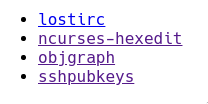
\includegraphics[]{../Pictures/overview.png}}
\caption{Overview of rebuild packages}%
\label{fig:rebuild-overview} 
\end{figure}

\begin{figure}[H]
\center{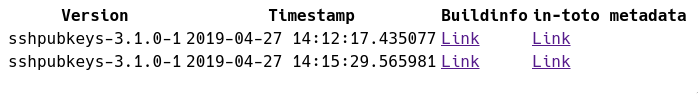
\includegraphics[width=\textwidth]{../Pictures/sources-view.png}}
\caption{Overview of the rebuild submissions}%
\label{fig:submission-overview} 
\end{figure}

The website as shown on Figure~\ref{fig:rebuild-overview} and
Figure~\ref{fig:submission-overview} displays the finished webserver for the
initial rewrite of the visualizer. The resulting code and webpage maintains
compatibility of the existing visualizer and enables us to continue implementing
further improvements on the API.

\subsection{Second Iteration: Merkle Tree}%
\label{sub:merkle_tree}
The second iteration focuses on implementing Merkle trees into the visualizer.
These will create the foundation of the transparency log in the upcoming
iterations for this project.

These will be implemented alongside of the reimplementation of the visualizer,
and the current structure of the code. We will take a look at the challenges of
implementing this correctly along with making sure the proofs are correctly
implemented to support a transparency log.

\subsection*{Goals}%
\label{sub:second_iteration_goals}
The goals of this iteration is to make sure the Merkle tree operated properly.
For this to happen there needs to be validated proofs and a proper tree
generated when new items are added. We will also be writing a very simple output
where we can visualize the generated tree as a node graph. This will aid in
debugging the creation of the tree.

\begin{itemize}
    \item Implement the needed database models for the datastructure
    \item New items should be appended to the tree
    \item The tree should not be rebuilt for each append
    \item Audit proofs should be implemented
    \item Consistency proofs should be implemented
    \item Visualize the tree graph
\end{itemize}


\subsection*{Development}%
\label{sub:second_iteration_development}
The main challenge in this iteration is getting the underlying data model
correct. What we are trying to achieve is to implement a tree structure where
the hash of the leafs is hashed together to form a chain of checksums all the
way up to the tree root. The following algorithm to achieve this is described
below.

The development of this project will be done in a few stages. First we will take
a look at the underlying database model needed to construct the trees. Next up
is how to construct Merkle trees without rebuilding all interior nodes. We need
to have a way to append new nodes by rehashing the least amount of interior
hashes.

The next development challenge in this iteration is to make sure the proofs are
working. Without appropriate proofs, mainly audit proofs and consistency proofs
as described in Subsection~\ref{sub:certificate_transparency_log}. We will go
through the development of these features and make sure they are working before
moving on for the next iteration.

As noted in Subsection~\ref{sub:transparency_log_library} on
page~\pageref{sub:transparency_log_library}, we are utilizing the pymerkle 
library written by~\citeauthor{pymerkeltools} to aid in the creation of the
transparency log proof algorithms~\cite{pymerkeltools}. It should be noted that
this library does not provide a persistence storage outside of just storing the
plain text tree as a JSON structure in a file. Our goal is to reuse portions of
the library code, and adapt them to a tree structure backed by PostgreSQL to
provide the transparency log features. This allows us to have a proper backend
storage for the Merkle tree.


\subsection*{Database}%
\label{sub:database}
Since we have implemented the visualizer with SQLAlchemy, the idea is to
utilize the SQL backend to store the tree. This gives a few challenges on how to
structure the model when it comes to relationships. We need to traverse the
tree for the proofs developed later on, so the relationships bindings in the
model should be correct and be easy to differentiate.

\begin{listing}[H]
\begin{minted}[linenos,numbersep=5pt,frame=lines,framesep=2mm]{python}
class Node(db.Model):
    __tablename__ = "node"
    id = db.Column(
        db.Integer(), index=True, unique=True, primary_key=True, autoincrement=True
    )
    leaf_index = db.Column(db.Integer(), default=0)
    type = db.Column(db.String(10), nullable=False)
    hash = db.Column(db.String(128))
    created = db.Column(db.DateTime, nullable=False, default=datetime.utcnow)
    data = db.Column(JSONB)
    height = db.Column(db.Integer(), default=0)
    children_right_id = db.Column(db.Integer, db.ForeignKey("node.id"))
    children_left_id = db.Column(db.Integer, db.ForeignKey("node.id"))

    right = db.relationship("Node",
            foreign_keys='Node.children_right_id',
            uselist=False,
            backref=db.backref('children_right', remote_side=[id]))

    left = db.relationship("Node", 
            foreign_keys='Node.children_left_id',
            uselist=False,
            backref=db.backref('children_left', remote_side=[id]))

    children_id = db.Column(db.Integer, db.ForeignKey("node.id"))
\end{minted}
\caption{Node SQLAlchemy model}
\label{lst:node_model}
\end{listing}

Listing~\ref{lst:node_model} shows the model that was settled on. Each of the
fields serve a purpose in the current model. ``leaf\_index'' keeps track of what
position as leaf node it was inserted as. This is important when we start
constructing proofs as some of the lookups needs to know what leaf number 16 is.
``type'' denotes one of two things, ``data'' for leaf nodes or ``level'' for
interior nodes.  ``data'' is a leaf node that has the ``data'' field filled with
JSON. ``level'' has no ``data'' field, but does have both ``left'' and ``right''
filled with the appropriate child node. ``hash'' contains the hash of the
``data'' JSON object.

The relationship modeled was a bit difficult to get correctly modeled in SQL.
The intentions were to have one foreign key to bind the left and right
relationships to, but this turned out to be difficult to implement. The solution
was to have the ``left'' relationship bind to ``children\_left\_id'' and
``right'' bind to ``children\_right\_id''. This solves the problem of having the
relationship correctly modeled. To find the correct child node for the leaf and
interior node, we need to check both left and right to find the correct node.

\begin{figure}[htpb]
\centering
\begin{tikzpicture}
\Tree
[ .r
[ .n1   [ .l ]  [ .r ]  ]
[ .n2 ]
]
\end{tikzpicture}
\caption{Example for relationships}
\label{fig:relationship_example}
\end{figure}

In the example node relationship in Figure~\ref{fig:relationship_example} we can
demonstrate what the ORM described in Listing~\ref{lst:node_model} would end up
looking like. If we sit with the appropriate model for ``N1'' we have an
interior node with a parent, left and right relationship. The parent node ``r''
where we can peek at the values ``children\_left'' and ``children\_right''
values to find the correct node. To find the ``l'' and ``r'' leaf nodes in this
example we only have to check the ``left'' and ``right'' relationships
respectively.

We are keeping everything in the same table with the same model. There is no
inherent distinction between leafs, interior nodes and root nodes in this
implementation when it comes to the model except for what is specified in the
``types'' direction. To find the root node in this implementation we only have
to look for the last inserted ``level'' node.

\subsection*{Construct tree}%
\label{sub:construct_tree}
We now have the database model we can build the tree with. Since this system is
supposed to run over time, and might target thousands of nodes, we need to be
able to append to the tree without rebuilding the entire tree. This is a
tedious process and could very well take quite a while if the number of nodes
grows large enough.

The algorithm to build a tree, where all the interior nodes are hashed for every
new insertion involves counting the number of nodes to be hashed. If this is an
odd number, promote the last node in this list to the next step. Now we take two
and two nodes and hash them together, left to right. This creates interior nodes
we call ``levels''. When this is done, we start from the beginning, and the
current set of interior nodes are the nodes we operate on.

This is a tedious process and does not scale very well over time. What we do
need is an algorithm that only rehashes the changed interior nodes.

The algorithm for this involves figuring out all the loose subroots of the tree.
This approach to append new nodes has been described in the original paper
by~\citeauthor{182788} where they calculate frozen subroots down on the left
side of the tree until the appropriate subroot is reached~\cite{182788}.

Our implementation is as follows; we take the count of all leaves in the tree and
use them to calculate the largest complete subtree in the Merkle tree, and
remove this from the count.  What we are left with are all the nodes in surplus
on the right hand side of the tree.

We can then walk down the tree on the left side, append the current node on the
path, and then do the same calculation with the nodes in surplus. We then know
the next complete subtree in the chain, remove the amount of nodes the complete
subroot has from the count, append the node and walk down. We continue this
until we reach 0 loose nodes, in which case we are at the node we are supposed to
append the new node too. The chain of appended nodes upwards is the list of
nodes we need to append with to rehash all of the interior nodes of the tree.

The resulting code takes the new node that is going to be appended, and hashes
it in the with the most recent node, then walks up the chain. This only rehashes
the interior nodes of the tree that needs to be rehashed. This lets us very
easily reach a fast append-only Merkle tree implementation backed by an SQL
database.


\subsection*{Cryptographic attack mitigation}%
\label{sub:mitigate_attack}
When constructing hashes we need to consider the two sources of information we
are essentially hashing. If the node is a leaf we need to hash the JSON data
structure. This is done by taking the keys and values in the JSON structure and
hashing them together in order. If the node is an interior node, this step is
omitted and the hash consists of the hash of the left and right nodes as shown
in Listing~\ref{lst:node_hashing_strategy}. The result of this is the
appropriate hash for the node.

\begin{listing}[H]
\caption{Node hashing strategy}
\label{lst:node_hashing_strategy}
\begin{equation*}
H\{\text{NodeType},\ \text{LeftNode},\ \text{RightNode}\}
\end{equation*}
\end{listing}

There are a few attacks one can do in practice on any data structure that uses
cryptographic hashes. Since the same output always returns the same value, they
are prone to what is called a ``second preimage'' attack. If the
attacker knows the input, they can re append the values, and create the same hash
in the tree.  This can allow the construction of malicious data or open up for
other venues of attack~\cite{rfc4270}.

To mitigate this, a certificate transparency log appends a null byte value for
leafs, and a 1 byte value for levels in the tree. This makes sure that we can't
replay previous data as there are always some values being appended. In our
implementation we append ``data'' and ``level'' as the prefix in the hashed
value. This serves the same purpose as the certificate transparency logs.


\subsection*{Graphviz}%
\label{sub:graph_merkle_tree}
To validate that we are getting the correct association and relationships when
appending new elements, one of the important things to get is a visualization of
the currently constructed Merkle tree. To aid the discovery of problematic
nodes, the first 10 letters of the hash is printed with the node to easily find
the affected node and aid debugging.

To do this we loop through all of the nodes in the tree. We print out the left,
and right parent of the node in a format that is compatible with the Graphviz
tool to generate pictures~\cite{Ellson01graphviz}. The output found in
Listing~\ref{lst:graphviz-test} enables us to produce the PDF picture in
Figure~\ref{fig:graphviz_pdf} by supplying the output to ``dot -Tpdf''.

It should be noted that when trees get sufficiently large, the graph itself is
of less value when debugging. It is hard to get a good overview when the tree
reaches around 60 nodes as the generated trees are spacious. Not enough time was
invested trying to fiddle with the style got a proper display when the trees
grow large. However, they did aid in early debugging when trees were sparse.

%TC:ignore
\begin{listing}[H]
\caption{Example graph of a generated tree}
\label{lst:graphviz-test}
\begin{minted}{bash}
$ curl 127.0.0.1:5000/api/log/tree/graphviz                        
graph graphname {
labelloc="t";
label="Nodes: 4";
"9A565DAB05" -- "B439C9F4B0";
"9A565DAB05" -- "730212F389";
"B439C9F4B0" -- "47A2AB3D2E";
"B439C9F4B0" -- "648D1817A3";
"730212F389" -- "92EF30AD83";
"730212F389" -- "1E94F9FDE4";
}
\end{minted}
\end{listing}
%TC:endignore

\begin{figure}[H]
\centering
\includegraphics[width=\textwidth]{../Diagrams/graph.pdf}
\caption{Graphviz visualization}
\label{fig:graphviz_pdf}
\end{figure}


\subsection*{Audit proof}%
\label{sub:audit_proof_implementation}
Audits proofs are important as they prove whether or not a given leaf is part of
the tree. They are used to validate that the data on the leaf is actually part
of a Merkle tree. The implementation of this is fairly straight forward as we
have implemented the database structure in a succinct manner.

The audit proof needs the id, or the hash of the node that should have the audit
proof generated. When we have the node, we essentially traverse the children of
the node. We then check on what side of the child the parent node is on. If it's
on the left side, we fetch the right node on the next child. This node is
appended to the list with the keyword ``RIGHT''. If it's on the right side, we
fetch the left node on the child. This node is appended to the list with the
keyword ``LEFT''. We then traverse to the next child and continue the path
upwards until the root node is reached, which has no child node.

When all the nodes are appended to a list, with the correct side expressed we
have a complete list of all the nodes needed. We can then append the current
root node to the response and let users hash the path and recreate the current
root node.

The appropriate JSON response for an example tree can be found in
Listing~\ref{lst:audit proof}. For the sake of being terse, some auxiliary
fields have been omitted in this example. In this case, to recreate the root
found in the top of the JSON output, we would just have to hash the ``path'' as
given and append the hash on the correct side of the previous hash.

\subsection*{Consistency proof}%
\label{sub:consistency_proof_implementation}
Consistency proofs are very similar to audit proofs, however they carry another
important property. They allow us to follow the path from a given known signed
Merkle tree root to the current new one. They are important to make sure we are
capable of tracing a path from the last known tree root we have, and to the
current one. 

To achieve this we need in practice two things; a known signed tree root and the
number of leafs present at this tree root. The current algorithm does this in
two steps. Procure the subroots needed to recreate the previous signed tree
root, then use these to recreate a path to the current tree root. 

The way to do this is to take the number of leaf nodes present in the input we
are given. We can use this to figure out all the expected complete subtrees in
the binary tree. These are represented as the expected heights of the given
roots. We can then take the heights, and start from the first leaf, move up the
tree until the root of the largest complete subtree is found. Then we know how
many leafs we have to move forward until we can start to climb the next subtree.

Once this is done with all the found heights, we have all the needed roots to
recreate the previous Merkle tree root. This can be checked by taking the
previous tree root which is given as the input and do at the same hash
concatenation as we do with the audit proof. If this value is as expected, we
can continue recreating the path to the current tree root.

Here we take each of the previous subroots and move up the tree until we reach
the current tree root. We end up with two paths. One consisting of the previous
subroots, and one of the remaining interior nodes we need to complete the path
to the Merkle tree root.

\subsection*{Results}%
\label{sub:second_iteration_results}
The second iteration was all about finishing up the Merkle tree approach so we
can construct a transparency log. The result has been a great deal of code to
make sure the tree works, and the properties and paths are generated correctly.
We have also made some debug utilities to make sure we have generated a well
formed binary tree, and no nodes are generating poor relationships.

\begin{table}[H]
\footnotesize
\centering
\settowidth\tymin{\textbf{Description}}
\setlength\extrarowheight{2pt}
\begin{tabulary}{1.0\textwidth}{|l|L|l|L|}
\hline
    \textbf{Endpoint} & 
    \textbf{Type} & 
    \textbf{Parameters} & 
    \textbf{Description} \\
\hline
    /api/log/stats & GET & & Statistics from the current tree \\ \hline
    /api/log/graphviz & GET & & Outputs the current tree in the dot format \\ \hline
    /api/log/root & GET & & Gets the latest tree root \\ \hline
    /api/log/tree/append & POST & JSON object & Appends a JSON object to the tree \\ \hline
    /api/log/tree/id/<id> & GET & & Gets the given Node object from the database with '``id''\\ \hline
    /api/log/tree/hash/<hash> & GET & & Gets the given Node object from the database with ``hash''\\ \hline
    /api/log/tree/leaf/<id> & GET & & Gets the given leaf from the database with matching ``leaf\_index''\\ \hline
    /api/log/tree/validate/id/<id> & GET & & Gets the audit proof for a leaf matching the given ``id''\\ \hline
    /api/log/tree/validate/hash/<hash> & GET & & Gets the audit proof for a leaf matching the given ``hash''\\ \hline
    /api/log/tree/consistency & POST & ConsistencyQuery & Provides the consistency proof for the given query\\ \hline
\end{tabulary}
\caption{Second Iteration: Transparency log API}
\label{api:transparency_log}
\end{table}

The Listing~\ref{api:transparency_log} shows the complete API that was designed
to along with the code base. This API lets us add arbitrary JSON objects to the
Merkle tree, and to inspect these nodes and verify them with an audit proof or
consistency proof.

The API allows for inspection of the tree with graphviz, along with also
inspecting individual interior nodes and leafs. It gives endpoints for the most
important features, namely the audit proof and the consistency proof.

The goals stated in the beginning of this iteration have been met. 

An appropriate database model has been constructed, and given us the needed
relationships between nodes to form a tree, and effectively ports the needed
algorithms to this tree structure. By lifting some code from the pymerkle
library we are able to create append-only trees without having to rehash all
interior nodes of the Merkle tree.

We are also capable of visualizing the created tree with graphviz for easier
debugging when dealing with the Merkle tree and detecting poor relationship
building and find other issues in the data structure.

To test this we are going to take a look at creating Merkle trees, issue audit
proofs, consistency proof and use the hashing scheme earlier to recreate root
hashes. This will help us prove a well functioning transparency log can be
achieved.

\begin{figure}[H]
\centering
\includegraphics[width=0.5\textwidth]{../Diagrams/4_tree.pdf}
\caption{Graphviz visualization of tree}
\label{fig:graph}
\end{figure}


Figure~\ref{fig:graph} shows the constructed Merkle tree. The first level is the
hash of all the leaf nodes which is currently some simple mock data in the JSON
structure for testing purposes. There is a total of 3 interior nodes, where the
top one is the Merkle tree root. Our goal is to test the appropriate proofs and
make sure we are getting back the appropriate nodes. These will help us make
sure we can reconstruct the root node in the tree.

\begin{figure}[H]
\centering
\subfloat[Validation proof nodes]{
\label{fig:validate_proof_tree}%
\includegraphics[width=0.46\textwidth]{../Diagrams/4_tree_validate.pdf}
}
\qquad
\subfloat[Consistency proof nodes]{
\label{fig:consistency_proof_tree}%
\includegraphics[width=0.46\textwidth]{../Diagrams/4_tree_consistency.pdf}
}
\caption{Proof nodes}
\label{fig:test_proof}
\end{figure}

Figure~\ref{fig:test_proof} shows the needed nodes for the different proofs.
They have been artificially colored in red after being fetched from our graphviz
API endpoint. The red color marks the needed nodes to construct the tree node
for each appropriate proof. 

It should be noted that while annotating the output graphs I discovered that the graphviz
output as displayed in Subsection~\ref{sub:graph_merkle_tree} is inherently
unordered, at least for complete subtrees. Incomplete subtrees would always be
output on the right hand side of the graph, but graphviz does not guarantee
any ordering of the internal subtrees. That means the graph as shown in these
examples does not completely represent the ordering of the internal tree, but
this has no bearing on the result of the generating paths at all. It's mostly a
minor inconvenience.

The proofs in Figure~\ref{fig:test_proof} are focused on leaf number two, in the
displayed graph leaf number three. A bit hard to follow, but we will endure!

\begin{listing}[H]
\caption{Path structure}
\label{lst:Path structure}
\begin{equation*}
    [(\text{Side},\ \text{NodeObject}),\ (\text{Side},\ \text{NodeObject})\ \dots]
\end{equation*}
\end{listing}

The way the path proofs are structured is a JSON object in a structure like
shown on listing~\ref{lst:Path structure}. We have tuples with two elements. The
first specifies the side which the hash should be concatenated on, this can
either be ``LEFT'' or ``RIGHT''. The node object is the JSON structure we get
from the Node object as defined in the ORM model.

\begin{listing}[H]
\caption{Code for validating path}
\label{lst:hashing algorithm}
\begin{minted}[linenos,numbersep=5pt,frame=lines,framesep=2mm]{python}
def validate_chain(root, chain):
    if not chain:
        return True
    chain = chain[:]
    s = chain.pop(0)[1]["hash"]
    for node in chain:
        h = hashlib.sha512()
        if node[0] == "LEFT":
            h.update(("level"+node[1]["hash"]+s).encode('utf-8'))
        if node[0] == "RIGHT":
            h.update(("level"+s+node[1]["hash"]).encode('utf-8'))
        s = h.hexdigest()
    return root["hash"] == s
\end{minted}
\end{listing}

To concatenate so we achieve the present root node, we need a function to hash
each of the tuples on the correct side. The Listing~\ref{lst:hashing algorithm}
displays this algorithm used in this project. There are a few important points.

The lines 2 and 3 deal with the possible issue of having an empty list hashed.
This is more of a short circuit in the case we are dealing with empty paths.
Line 4 explicitly deals with the fact that Python is designed to be
pass-by-reference. Any modifications on the path when we pop off items to create
the hash will affect any code holding the reference. We thus copy the list to
make sure no references are modified. The rest of the code is all about
concatenating the strings on the correct side of the nodes to create the hash.


%TC:ignore
\begin{listing}[H]
\caption{JSON for audit proof}
\label{lst:audit proof}
\begin{minted}[numbersep=5pt,frame=lines,framesep=2mm]{json}
$ curl 127.0.0.1:5000/api/log/tree/validate/id/2
{"root": {
    "id": 8,
    "type": "level",
    "hash": "f9c955f75e...",
    "right": "ffcd54e492...",
    "left": "b9464656e8..."},
  "path": [
    ["RIGHT", {
        "id": 2,
        "type": "data",
        "hash": "04f757137e...",
        "parent": "b9464656e8...",
        "data": {"data": "Datablock-1", "name": "Name-1"}}],
    ["LEFT", {
        "id": 1,
        "type": "data",
        "hash": "6375bda107...",
        "signature": "8acfc7f730...",
        "parent": "b9464656e8...",
        "data": {"data": "Datablock-0", "name": "Name-0"}}],
    ["RIGHT", {
        "id": 7,
        "type": "level",
        "hash": "ffcd54e492...",
        "right": "74a7004f39...",
        "left": "2ba5b40dbe...",
        "parent": "f9c955f75e..."}]],
  "validation": true}
\end{minted}
\end{listing}
%TC:endignore

Listing~\ref{lst:audit proof} is the audit proof we need for leaf number 2 when
calling the API. It should be noted that we do validate the path on the server
side and return the result in the ``validation'' field, but clients shouldn't
trust this value blindly. This do make for easy debugging when we are running
this locally. We are also abbreviating some of the structure and hashes for the
sake of keeping things terse.

The Figure~\ref{fig:validate_proof_tree} on page
\pageref{fig:validate_proof_tree} is the audit tree with the appropriately
highlighted nodes, and the same nodes are found by the audit endpoint and a path
to the root node is correctly generated. This can be verified running the given
structure with the previously mentioned hash function.

In our case we can also trust the initial validation done by the server, as it
uses the same function to hash and compare the root node. However our client
implementation should not rely on this.


%TC:ignore
\begin{listing}[H]
\caption{JSON for consistency proof}
\label{lst:consistency proof}
\begin{minted}[numbersep=5pt,frame=lines,framesep=2mm]{json}
$ curl 127.0.0.1:5000/api/log/tree/consistency/2
{"root": {
    "id": 8,
    "type": "level",
    "hash": "f9c955f75e...",
    "right": "ffcd54e492...",
    "left": "b9464656e8..."},
  "leaf nodes": 4,
  "inclusion": true,
  "consistency": true,
  "path": [
    ["RIGHT", {
        "id": 7,
        "type": "level",
        "hash": "ffcd54e492...",
        "right": "74a7004f39...",
        "left": "2ba5b40dbe...",
        "parent": "f9c955f75e..."}],
    ["LEFT", {
        "id": 3,
        "type": "level",
        "hash": "b9464656e8...",
        "right": "04f757137e...",
        "left": "6375bda107...",
        "parent": "f9c955f75e..." }]]}
\end{minted}
\end{listing}
%TC:endignore

Listing~\ref{lst:consistency proof} displays the consistency proof. It is
considerably smaller then the audit proof as we are only dealing with the
subroots. Since we are dealing with a rather small tree, it is not the best
situation to show off a consistency proof, as one subroot of the two is a
previous Merkle tree root. Thus we are only getting two in return we need to
hash together. 

However, as shown on Figure~\ref{fig:consistency_proof_tree} on
page~\pageref{fig:consistency_proof_tree} we are returned the correct tree roots
for the proof and thus we have implemented the needed proofs.

In Section~\ref{ch:evaluation} on page~\pageref{ch:evaluation} we are going to
investigate and test the transparency log implementation further.

\subsection{Third Iteration: Tree root signing}%
\label{sub:tree_root_signing}
One essential part of Merkle trees as implemented
by~\citeauthor{b.-laurie-a.-langley-e.kaster-google-2013} in certificate
transparency logs is the ability to have tree-roots
signed~\cite{b.-laurie-a.-langley-e.kaster-google-2013}. This lets us verify
with public key cryptography that the tree-root was created by the given
transparency log. In this chapter we will go through how this is implemented.

\subsection*{Goals}%
\label{sub:third_iteration_goals}

The goals of this iteration is to create the needed code to create and verify
signatures on tree nodes.

\begin{itemize}
    \item Initialize signing keys
    \item Sign every tree root created by the log
    \item Verify the signature
\end{itemize}

\subsection*{Development}%
\label{sub:third_iteration_development}
For the development of this feature we are utilizing the securesystemslib from
New York University's' secure systems lab~\cite{securesystemslib}. It's a
library with a collection of easy-to-use primitives to deal with encryption,
decryption and signature verification on data for Python. Utilizing this library
makes it trivial to implement the needed signature functionality in a short and
concise manner.

\begin{listing}[H]
\caption{Glue code for ``securesystemslib''}
\label{lst:securesystemslib_glue}
\begin{minted}[linenos,numbersep=5pt,frame=lines,framesep=2mm]{python}
PASSWORD = "123"
KEY_NAME = "ed25519_key"

def init_keys():
    if not os.path.isfile(KEY_NAME):
        generate_and_write_ed25519_keypair(KEY_NAME, password=PASSWORD)

def get_private_key():
    init_keys()
    return import_ed25519_privatekey_from_file(KEY_NAME, password=PASSWORD)

def get_public_key():
    init_keys()
    return import_ed25519_publickey_from_file(KEY_NAME+'.pub')

def sign_data(data):
    return create_signature(get_private_key(), data)

def verify_data(signature, data):
    return verify_signature(get_private_key(), signature, data)
\end{minted}
\end{listing}

The implementation itself consists of a file for the needed code to ease the key
creation for the rebuilder. For the sake of ease, we don't consider problems
such as password strength for the signing key as the main focus is on the
transparency log implementation. In this implementation the password is hard
coded to ``123'', which is admittedly a poor password. For the cryptography,
elliptic curves are used instead of the traditional RSA algorithm. The reason is
that elliptic curves needs less bits to produce equally strong keys. We then end
up with faster and smaller signatures.

These auxiliary functions makes it trivial to further implement the tree root
signing in the model.

\begin{listing}[H]
\caption{Additions to the Node model}
\label{lst:node_tree_root_signature}
\begin{minted}{diff}
@@ -21,10 +22,10 @@ class Node(db.Model):
     leaf_index = db.Column(db.Integer(), default=0)
     type = db.Column(db.String(10), nullable=False)
     hash = db.Column(db.String(128))
+    signature = db.Column(db.String(128))
     created = db.Column(db.DateTime, nullable=False, default=datetime.utcnow)
     data = db.Column(JSONB)
     height = db.Column(db.Integer(), default=0)
\end{minted}
\end{listing}

In Listing~\ref{lst:node_tree_root_signature} we can see the additions to the
``Node'' model from Listing~\ref{lst:node_model} page~\pageref{lst:node_model}.
This enables us to store the signature string in the database model for future
use when creating tree roots.

\begin{listing}[H]
\caption{Additions to the append function}
\label{lst:append_tree_root_signing}
\begin{minted}{diff}
@@ -166,7 +168,9 @@ def append(data):
     for node in reversed(subtrees):
         new_parent = create_level_node(node, new_node)
         new_node = new_parent
+    signature = sign_data(new_node.hash)
+    new_node.signature = signature["sig"]
     db.session.commit()
     return ret
\end{minted}
\end{listing}

Listing~\ref{lst:append_tree_root_signing} shows the additions made to the
``append'' function to support signed tree roots. Since the last ``new\_node'' is
the new tree root, we only sign the hash of this node. This is enough to
implement tree root signing in the current implementation of the visualizer.

\subsection*{Results}%
\label{sub:third_iteration_results}

The results of this iteration is two new endpoints and some new code to help with
signing tree roots in the transparency log. The resulting API endpoints can be
found in Table~\ref{api:crypto_api} which shows the newly created endpoints.

\begin{table}[H]
\footnotesize
\centering
\settowidth\tymin{\textbf{Description}}
\setlength\extrarowheight{2pt}
\begin{tabulary}{1.0\textwidth}{|l|L|l|L|}
\hline
    \textbf{Endpoint} & 
    \textbf{Type} & 
    \textbf{Parameters} & 
    \textbf{Description} \\
\hline
    /api/crypto/key & GET & & Outputs the key object used by the library \\ \hline
    /api/crypto/validate & POST & Tree root hash and signature & Validates the tree root to the public key \\ \hline
\end{tabulary}
\caption{Third Iteration: Crypto API}
\label{api:crypto_api}
\end{table}

The usage of the endpoints is fairly straight forward. We can call the generated
signing key with ``/api/crypto/key'' as shown in
Listing~\ref{lst:display-generated-public-key}. Which enables us to verify the
signature on the client side instead of on the server side if we need to do
that.

%TC:ignore
\begin{listing}[H]
\caption{Display generated public key}
\label{lst:display-generated-public-key}
\begin{minted}{bash}
$ curl 127.0.0.1:5000/api/key
{
  "keytype": "ed25519",
  "scheme": "ed25519",
  "keyid": "25a16bb3a3...",
  "keyid_hash_algorithms": [
    "sha256",
    "sha512"
  ],
  "keyval": {
    "public": "7623ba359c..."
  }
}
\end{minted}
\end{listing}
%TC:endignore

To verify a tree root on the server side, we can provide the output from
``/api/log/tree/root'' from Table~\ref{api:transparency_log}, and forward this
to ``/api/crypto/verify''. In the example from
Listing~\ref{lst:test-verify-endpoint}, we have provided a minimal tree root
JSON object to display a successful verification of a tree root on the server
side.

%TC:ignore
\begin{listing}[H]
\caption{Test of the verify endpoint}
\label{lst:test-verify-endpoint}
\begin{minted}{bash}
$ curl --header "Content-Type: application/json" \
  --request POST \
  --data '{"hash": "21e0b13a6f...", \
           "signature": "832510c0188..."}' \
  127.0.0.1:5000/api/crypto/verify
{
  "status": "ok",
  "verified": true
}
\end{minted}
\end{listing}
%TC:endignore


\subsection{Fourth Iteration: Transparency log overlay}%
\label{sub:transparency_overlay}
In this section we are going to create an abstraction over the values we insert
into the Merkle tree. So far we have only been using testing values to test the
correctness of the tree. But we are after all going to record the submissions
from the rebuilder and append them to the log. We also need to expose a new API
to the APT transport which we need to integrate with at a later point.

We want to have some enforced properties to see how we can implement
abstractions on the values. We can't remove entries once they are on the
transparency log, but we might want to retain the property of revoking package
submissions. This could be because of build environment compromises, or security
advisories from the parent distribution.

\subsection*{Goals}%
\label{sub:fourth_iteration_goals}

The goals for this iteration are as follows;

\begin{itemize}
    \item We should have well defined entry formats
    \item We should be able to find package submissions
    \item We should be able to revoke package submissions
\end{itemize}

\subsection*{Development}%
\label{sub:fourth_iteration_development}
First we need to figure out what data we are dealing with. Let us start off by
defining one item appended on the tree as an ``Entry''. An entry should always
contain two key pieces of information, namely package name and version. This is
important to retrieve them at a later point so we are capable of doing the
package verification with the APT package manager.

Once we have established this we need to figure out what sort of entries we are
dealing with. We are going to deal with two actions, accepting submissions from
the rebuilder, which we will call inclusions, and revocations of said
submissions. 

\begin{listing}[H]
\caption{Entry definitions}
\label{lst:entrydefinitions}
\begin{minted}[linenos,numbersep=5pt,frame=lines,framesep=2mm]{python}
inclusion = {"type": "inclusion",
             "package": pkg_name,
             "version": version,
             "linkmetadata": metadata.read().decode("utf-8"),
             "buildinfo": buildinfo.read().decode("utf-8")}

revoke = {"type": "revoke",
          "package": pkg_name,
          "version": version,
          "hash": hash,
          "reason": reason}
\end{minted}
\end{listing}

Listing~\ref{lst:entrydefinitions} displays Python code to illustrate the
two entries we are going to be dealing with on this transparency log. We have
the ``inclusion'' entry which lists the package name and version. This is a
common field assumed for all entries, along with the appropriate files that
contain the buildinfo, which contains the record for the build environment. 

We also have linkmetadata, which is the in-toto metadata needed for the client
verification later on. This denotes that the package and the files has been
rebuilt and is a submission.

The other entry we will be dealing with is a ``revoke'' entry. This denotes an
inclusion which has been marked as bad. We will be using these entries to mask
inclusion entries on the client side. This contains two fields. The ``hash''
field denotes the hash of the Merkle tree object containing an inclusion entry.
The next field is ``reason'' which can contain an optional message as to why the
given inclusion has been revoked.

To implement support for this we are going to take the submission endpoint from
the first iteration on Subsection~\ref{sub:first_iteration_development} on
page~\pageref{sub:first_iteration_development}.

Extending the previous ``/new\_build'' endpoint, where we are creating the
needed ``Package'' and ``Version'' models for database insertion, we now also
append the relevant information to the transparency log. This is fairly
straightforward as we only need to construct the ``inclusion'' dictionary and
insert it as JSON into the database.

\begin{listing}[H]
\caption{Fetch entries}
\label{lst:fetch_entries}
\begin{minted}[linenos,numbersep=5pt,frame=lines,framesep=2mm]{python}
@app.route("/api/rebuilder/fetch/<name>/<version>")
@json_response
def rebuilder_fetch(name, version):
    records = (db.session.query(Node)
            .filter(Node.data.op('->>')('package') == name)
            .filter(Node.data.op('->>')('version') == version)
            .order_by(Node.created.desc())
            ).all()
    return [[rec.to_json(), audit_proof(rec)] for rec in records]
\end{minted}
\end{listing}

We also need to fetch all entries on the database given a package name and
version. PostgreSQL has dedicated JSON support in their database, which our
model defined on Listing~\ref{lst:node_model} on page~\pageref{lst:node_model}
has implemented for the data field. What we can now do is use native PostgreSQL
filters on the JSON as seen on Listing~\ref{lst:fetch_entries}. This allows us
to easily filter through all entries and return them easily for the REST API.

For each of the entries a corresponding audit proof needs to be fetched. To
lessen the burden on the client, we append this proof to the response. This
allows us to not having to implement the audit proof fetching and validation 

When it comes to having a ``revoke'' entry, we need to have a few
considerations in place. As input we need the hash of a node on the Merkle
tree with a ``inclusion'' entry. Currently we don't want to publish revocations
of any objects, as further entries could be implemented in the future. What we do
is that we look up the hash, get the object and verify the type of the entry
before submitting the revoke entry on the object.

\subsection*{Results}%
\label{sub:fourth_iteration_results}
The results of this iteration is the last and final API. This iteration
completes the work on the rewrite of the visualizer and provides us with a new
API that will be used for the upcoming APT integration.

\begin{table}[hbtp]
\footnotesize
\centering
\settowidth\tymin{\textbf{Description}}
\setlength\extrarowheight{2pt}
\begin{tabulary}{1.0\textwidth}{|l|L|L|L|}
\hline
    \textbf{Endpoint} & 
    \textbf{Type} & 
    \textbf{Parameters} & 
    \textbf{Description} \\
\hline
    /api/rebuilder/submit & POST$^1$ & metadata, buildinfo& Implements something heyho lets go \\  \hline
    /api/rebuilder/revoke& POST$^1$ & leaf hash, reason, signature& Revokes the leaf with a reason  \\  \hline
    /api/rebuilder/fetch/<name>/<version>& GET & & Gets the entries for the given package \\  \hline
\end{tabulary}
\footnotesize{$^1$ Behind authentication}\\
\caption{Fourth Iteration: Overlay API}
\label{api:Overlay API}
\end{table}

The API as listed in~\ref{api:Overlay API} gives us the ability to submit new
rebuilds, and at a later point revoke them if needed. All of this is stored on
an abstracted API where we don't have to deal with the transparency log
directly.

\begin{listing}[H]
\caption{Example of rebuild submission}
\label{lst:rebuild_submission_curl}
\begin{minted}{bash}
$ curl -F "metadata=@metadata" -F "buildinfo=@buildinfo" \
  127.0.0.1:5000/api/rebuilder/submit
{"status": "ok",
  "node": {
    "id": 1,
    "hash": "9432b4df00...",
   ...}}

$ curl 127.0.0.1:5000/api/log/tree/leaf/index/1
{"id": 1,
  "hash": "9432b4df00...",
  ...}
\end{minted}
\end{listing}

Listing~\ref{lst:rebuild_submission_curl} shows how we can submit a rebuild,
consisting of the buildinfo file and the linkmetadata file, to the submit
endpoint. This will create the appropriate models, and append it to the
transparency log as shown when we call it with the appropriate index.

%TC:ignore
\begin{listing}[H]
\caption{Example of rebuild revoke}
\label{lst:rebuild_revoke_curl}
\begin{minted}{bash}
$ curl -XPOST --header "Content-Type: application/json" \
  --data '{"hash":"9432b4df00...","reason":"testing"}' \
  127.0.0.1:5000/api/rebuilder/revoke
{"status": "ok",
  "node": {
    "id": 2,
    "type": "data",
    "hash": "d22c2446cb...",
    "parent": "e5a6599214...",
    "data": {
      "hash": "9432b4df00...",
      "type": "revoke",
      "reason": "testing",
      "package": "lostirc",
      "version": "0.4.6-4.2"
    }}}
\end{minted}
\end{listing}
%TC:endignore

Listing~\ref{lst:rebuild_revoke_curl} enables us to revoke the inclusion on the
tree and also allows us to state the reason for the revocation of the inclusion.
This evidently works fine and allows us to fetch all of the entries on the test
package. We are currently using a previously rebuilt package with a corresponding
linkmetadata file. The package is called ``lostirc'' and the version is
``0.4.6-4.2''

%TC:ignore
\begin{listing}[H]
\caption{Example of fetching entries}
\label{lst:rebuild_fetch_curl}
\begin{minted}{bash}
$ curl 127.0.0.1:5000/api/rebuilder/fetch/lostirc/0.4.6-4.2
[{"id": 2,
   "type": "data",
   "hash": "d22c2446cb...",
   "data": {
     "hash": "9432b4df00...",
     "type": "revoke",
     "reason": "testing",
     "package": "lostirc",
     "version": "0.4.6-4.2"}},
  {"id": 1,
   "type": "data",
   "hash": "9432b4df00...",
   "data": {
     "type": "inclusion",
     "package": "lostirc",
     "version": "0.4.6-4.2"
     ...}}]
\end{minted}
\end{listing}
%TC:endignore

Listing~\ref{lst:rebuild_fetch_curl} shows how entries are gotten in descending
order of creation. First the revocation entry, then the inclusion entry. This
allows us to read each entry subsequently in order, and act on the next elements
according to previous entries. We can also see how we are capable of fetching
multiple inclusion proofs for the same package as we are only dealing with the
package name and the package version.

This API is flexible and can be extended to include multiple entries in the
future. We will now attempt to integrate them into the APT package handler.


\subsection{APT Transport integration}\label{sec:apt_transport}
So far in this thesis we have implemented the server side of this software. Now
comes the client side which will do the package verification towards the
visualizer.  The current rebuilder system as implemented before this thesis,
there was an integration with the APT package manager for Debian written for
this. The purpose of this integration is to have a process which let APT  
download the appropriate package, but in a way where we can do additional
verification.


\begin{figure}[H]
  \centering
  \begin{sequencediagram}
    \newthread{A}{HTTP client}{}
    \newinst[1]{B}{intoto}{}
    \newinst[2]{C}{APT Server}{}
    \begin{messcall}{A}{100 Capabilities}{C}
        \begin{messcall}{C}{601 Configuration}{A}\end{messcall}
        \begin{messcall}{C}{600 URI Acquire}{A}\end{messcall}
        \begin{messcall}{A}{200 URI Start}{C}\end{messcall}
            \begin{messcall}{C}{201 URI Done}{B}
                \begin{sdblock}{Rebuilder verify}{}
                    \begin{messcall}{B}{201 URI Done}{A}\end{messcall}
                \end{sdblock}
            \end{messcall}
    \end{messcall}
  \end{sequencediagram}
\caption{in-toto sequence diagram}
\label{fig:intoto_sequence_diagram}
\end{figure}

The sequence diagram in Figure~\ref{fig:intoto_sequence_diagram} shows the idea
behind this. When APT communicated with a package repository it will use a
binary for the communication between the client and the server. What we have is
an ``in-toto'' client which can be used as a drop-in replacement of the ``http''
one. We only forward between the client and the APT server until we see that a
package has been acquired, this is recognized when the ``201 URI Done'' message
is passed. This implies we have downloaded the package locally. We
man-in-the-middle this message and begin our verification process.

This process involves having configured one or more rebuilders we should be
communicating with in a configuration file. We will then request each of the
rebuilders on this list for the linkmetadata file. The verification step is
implemented with ``in-toto''. This involves a layout from in-toto which
describes the expected keys and the threshold that needs to be met for the
process to succeed. If the validation with the linkmetadata is approved, which
means the downloaded package has the same checksum as the signed layout says it
has, we will forward the ``201 URI Done'' message to the client APT and the
package will be installed.

The development in this section is to move the current implementation away from
the old API, which is a very simple file listing, to the transparency log
implementation.


\subsection*{Goals}%
\label{sub:apt_transport_goals}
For this integration we need to move the old API interactions to the new one. To
do this we need to implement a few things.

\begin{itemize}
    \item We need to store rebuilder tree roots
    \item We need to verify any signatures
    \item We need to verify the consistency proof
    \item Parse available entries
    \item We need to verify the audit proof of entries
    \item Validate with available metadata
\end{itemize}

An additional goal of the API is to validate the output without need to trust
any validations the rebuilder does.

\subsection*{Development}%
\label{sub:apt_transport_development}
To validate the downloaded packages against available linkmetadata, we need to
implement and support a few states. We can't just ask for the given entries, we
also need to validate the state of the Merkle tree with the consistency proof
from the Merkle tree. All of this should be done locally.

The steps needed are
\begin{enumerate}
    \item Have previous known Merkle tree state
    \item Fetch consistency proof and validate this proof
    \item Store new tree root in place of old tree root
    \item Fetch available entries on the given package
    \item Fetch audit proof for each entry and validate this proof
    \item Validate package -with any valid inclusion entries
\end{enumerate}

It should be noted that any validation step on tree nodes need to attempt to
recreate the hash appropriately. We also need to validate any signatures on
Merkle tree roots. Thus our additions to the ``in-toto'' transport amounts to 5
functions.

\begin{itemize}
    \item compare\_hash
    \item validate\_chain
    \item verify\_consistency
    \item store\_new\_tree\_root
    \item fetch\_rebuild
\end{itemize}

``compare\_hash'' will be our function making sure the node hash is correct. It
will take the parents and data directive as appropriate and calculate the hash
as a boolean value.  ``validate\_chain'' will utilize the ``compare\_hash''
function and make sure the given path for audit proofs and consistency proofs
are correct.  ``verify\_consistency'' will request the consistency proof and
build on top the previous functions. It will take the rebuilder, leaf count and
previous root and make sure the proof with the current tree root is signed along
with the path validating.

Once this is done we can store the new tree root locally with
``store\_new\_tree\_root''. This leaves us with fetching the current entries of
the given package and version which will be done with ``fetch\_rebuild''. It
will loop over any given entry, and mask any hashes where we have a ``revoke''
entry. We will also make sure the consistency proof of the given entry is
correct.

%TC:ignore
\begin{listing}[H]
\caption{Difference in ``intoto.py'' verification step}
\label{lst:intoto_changes}
\begin{minted}{diff}
@@ -563,21 +649,21 @@ def _intoto_verify(message_data):
       .format(len(global_info["config"]["Rebuilders"])))
   # Download link files to verification directory
   for rebuilder in global_info["config"]["Rebuilders"]:
-    # Accept rebuilders with and without trailing slash
-    endpoint = "{rebuilder}/sources/{name}/{version}/metadata".format(
-        rebuilder=rebuilder.rstrip("/"), name=pkg_name,
-        version=pkg_version_release)
-
-    logger.info("Request in-toto metadata from {}".format(endpoint))
 
     try:
-      # Fetch metadata
-      response = requests.get(endpoint)
-      if not response.status_code == 200:
-        raise Exception("server response: {}".format(response.status_code))
+      proof = verify_consistency(rebuilder)
+      if not proof:
+        raise Exception("Can't verify consistency on rebuilder {}".format(rebuilder))
+
+      store_new_tree_root(rebuilder, proof)
+
+      rebuild = fetch_rebuild(rebuilder.rstrip("/"), pkg_name, pkg_version_release)
+      if not rebuild:
+        raise Exception("No available rebuild from {}".format(rebuilder))
+
+      link_json = json.loads(rebuild["data"]["linkmetadata"])
 
-      # Decode json
-      link_json = response.json()
+      logger.info('{}'.format(link_json))
\end{minted}
\end{listing}
%TC:notignore

Listing~\ref{lst:intoto_changes} shows the difference in code for the
verification step in the transport after the initial implementation. This
implementation fetches from the new rebuilder API instead of the old one with
the least amount of intrusive code to the current project.

%TC:ignore
\begin{listing}[H]
\caption{File format for storing tree roots}
\label{lst:tree_root_store}
\begin{minted}{json}
{
    "http://127.0.0.1:5000": {
        "hash": "78f6bbe2f6...",
        "signature": "b8d0925acd...",
        "count": 15
    }
}
\end{minted}
\end{listing}
%TC:endignore

We have also included a new option in the configuration file for the APT 
transport. We need a way to store previous tree roots from multiple rebuilders,
so settled on a fairly simple JSON format which meets our needs fairly well.
Listing~\ref{lst:tree_root_store} shows the format which is a simple key value
format where we store the three important pieces of information. The hash of a
tree root, the signature of the tree root and the number of leafs present when
this tree root was the current version. We write this file as appropriate when
new tree roots are gathered.

The links to the source code of this can be found in
Appendix~\ref{appendix:apt-development-source} on
page~\pageref{appendix:apt-development-source}.

\subsection*{APT Transport Testing}%
\label{sub:apt_transport_testing}
For the testing part we are going to reuse the test setup written for the
original APT transport and make sure it has everything it needs to test towards
the new API.

The current test setup heavily relies on mocking three parts of this setup. The
APT client, the APT server and the rebuilder. All of these are mocked in an
attempt to only test the ``intoto'' transport. To test our new API we will
remove the rebuild mocking which the test setup utilizes. This enables us to
test the new rebuilder directly instead of utilizing a mock of the API.

First we need to modify the in-toto layout used for testing. The in-toto layout
is used for making sure thresholds of available, and good, linkmetadata exists for
the given package. The current test setup requires two good metadata files to
exist, this is because they are utilizing the test setup with two rebuilders to
make sure things work appropriately. In our case we only really care about the
``intoto'' transport communicating correctly with the new API. We modify the
linkmetadata for the tests to only account for one valid linkmetadata file, then
resign it with the correct key used in the setup with the ``in-toto-sign''
utility.

The next challenge is to make sure we are initializing the consistency proof
tree root correctly. To do this we make sure we are dealing with a reproducible
setup so the seeded Merkle tree root doesn't change between tests. We do this by
first initializing a Merkle tree with 10 elements. Then we pick one of these
roots which we will use to start off on our testing, in our case we went with
the Merkle tree root present when there was four leaf nodes for no particular
reason. We make sure we store this file, and copy it to the right location,
along with making sure the mock APT client has the configuration set to look for
this file.

The resulting test suite thus passes and we have managed to integrate the APT
transport with the new API. Appendix~\ref{appendix:apt_testing} on
page~\pageref{appendix:apt_testing} goes through the test setup of the APT 
transport and the resulting test suite run. This helps make sure the results are
reproducible.

\section*{Summary}\label{sec:development-summary}
In this section we have explained how the development of the new visualizer was
done. What we got is a new visualizer where we have support for transparency
logs and an extended API and code base to help further development in the
future.

We have also done the needed integration between the transparency log and
verified it works.

\blankpage
\end{document}
